\section{Wprowadzenie}

Niniejszy rozdział zawiera przegląd źródeł danych mogących służyć zarówno jako źródła zmiennych zależnych, jak i \textit{zmiennych pomocniczych} w estymacji pośredniej. Scharakteryzowano w nim w pierwszej kolejności badania reprezentacyjne będące podstawą publicznej informacji na temat dochodów ludności Polski. Następnie, uwzględniając przede wszystkim cel pracy, Przedstawiono spisy ludności, które stanowią cenne i bogate źródło \textit{zmiennych pomocniczych} dostępnych na niskich poziomach agregacji przestrzennej. W rozdziale znalazły się także informacje na temat rejestrów administracyjnych zawierających dane dotyczące ubóstwa i zjawisk pokrewnych. W ostatniej, czwartej części rozdziału nawiązano do nowych i coraz częściej wykorzystywanych w analizach zasobów danych określanych mianem Big Data. W dobie powszechnego dostępu do Internetu uwzględnienie możliwości pozyskania danych do estymacji pośredniej z innych, niestatystycznych źródeł staje się bowiem jednym z obowiązkowych etapów badania.

\section{Badania reprezentacyjne}

Podstawowym źródłem danych o warunkach życia ludności w Polsce są badania reprezentacyjne prowadzone przez Główny Urząd Statystyczny. Wśród nich najpoważniejszą rolę odgrywają: Badanie Budżetów Gospodarstw Domowych (BBGD) oraz Europejskie Badanie Dochodów i Warunków Życia (EU-SILC). Od roku 2011 w cyklu czteroletnim realizowane jest także nowe badanie GUS --- Badanie Spójności Społecznej (BSS). Ponadto należy także wspomnieć o przekrojowym badaniu Diagnoza Społeczna (DS) prowadzonym przez Radę Monitoringu Społecznego. W kolejnych podrozdziałach badania te zostaną szerzej scharakteryzowane.

\subsection{Badanie Budżetów Gospodarstw Domowych}

Badanie Budżetów Gospodarstw Domowych (BBGD) jest podstawowym źródłem o przychodach, rozchodach, spożyciu ilościowym żywności oraz innych aspektów warunków życia ludności. Dane pochodzące z badania wykorzystywane są m.in. do analizy poziomu życia gospodarstw domowych, obliczania wskaźników cen towarów i usług, określenia poziomu minimalnego wynagrodzenia oraz badania ubóstwa. Schemat zgodnie z którym obecnie realizowane jest Badanie Budżetów Gospodarstw Domowych obowiązuje od 1992 roku. Co miesiąc losowana jest próba składająca się z 3132 mieszkań. Badaniu podlegają wszystkie gospodarstwa domowe zamieszkujące wylosowane mieszkanie. W przypadku odmowy udziału w badaniu, gospodarstwo jest zastępowane przez jednostkę pochodzącą z tzw. próby rezerwowej. Rokrocznie w BBGD bierze udział około 37 tys. gospodarstw.

Mieszkania do badania losowane są na podstawie dwustopniowego schematu losowania przy wykorzystaniu operatu uwzględniającego podział terytorialny kraju (TERYT). W badaniu stosuje się model rotacji całkowitej z miesięcznym okresem wymiany próby. Oznacza to, że w każdym miesiącu badane są inne jednostki. Gospodarstwa domowe uczestniczące w badaniu są zobowiązane do rejestrowania swoich przychodów i rozchodów w tzw. książeczkach budżetowych przez cały miesiąc \citep{bbgd_met2011}.

Wyniki badania publikowane są w przekroju grup społeczno-ekonomicznych, według wielkości gospodarstwa domowego, miejsca zamieszkania (miasto/wieś), według typu biologicznego gospodarstwa domowego oraz według podstawowych grup potrzeb i asortymentów towarów. Wybrane statystyki takie jak wskaźnik miesięcznych dochodów rozporządzalnych, wskaźnik przeciętnych miesięcznych wydatków na 1 osobę czy wyposażenie w wybrane dobra trwałego użytkowania przedstawiane są w przekroju województw \citep{bbgd2016}. BBGD stanowi podstawę do opracowania publikacji GUS pt. ,,Ubóstwo w Polsce'' wydawanej z częstotliwością roczną \citep{ubostwo-gus2015}.

Koszt przeprowadzenia badania w 2016 roku według informacji zawartych w Programie Badań Statystycznych Statystyki Publicznej wyniósł 26 800 300 zł \citep{pbs2015}.

\subsection{Europejskie Badanie Dochodów i Warunków Życia}

Celem Europejskiego Badania Dochodów i Warunków Życia (EU-SILC) jest dostarczenie porównywalnych danych na temat osób i gospodarstw domowych dla krajów Unii Europejskiej. Pierwszy raz zostało ono przeprowadzone w 2003 roku, a dwa lata później wdrożono je w 25 krajach Unii Europejskiej. Badanie EU-SILC stanowi podstawowe źródło danych na temat dochodów, ubóstwa i wykluczenia społecznego. Otrzymane wyniki umożliwiają monitorowanie skutków działań podejmowanych w ramach programów mających na celu ograniczanie ubóstwa takich jak np. \textit{Europa 2020}. 

EU-SILC, podobnie jak Badanie Budżetów Gospodarstw Domowych, bazuje na dwustopniowym schemacie losowania próby. W pierwszym roku badania wylosowano około 24 tys. mieszkań. Następnie, wylosowane mieszkania podzielono na 4 rozłączne i równoliczne podpróby. Od 2006 roku jedna z podprób jest wykluczana, a na jej miejsce losuje się nową podpróbę. W badaniu EU-SILC próba rezerwowa nie jest dobierana i w związku z tym w przypadku odmowy udziału, mieszkanie nie jest zastępowane innym. W znacznym stopniu niekorzystnie wpływa to na liczbę przebadanych gospodarstw. Badanie EU-SILC jest realizowane techniką bezpośredniego wywiadu z respondentem zawsze w drugim kwartale każdego roku.

Zgodnie z założeniami badania, zmienne dochodowe nie powinny zawierać braków danych. W~związku z tym, że jest to informacja wrażliwa, którą respondent dzieli się niechętnie, konieczna jest imputacja danych. W badaniu EU-SILC stosowane są cztery różne metody: hot-deck, imputacja regresyjna z losowymi resztami empirycznymi, deterministyczna imputacja regresyjna oraz imputacja dedukcyjna. Zastosowanie tych technik umożliwia uzyskanie zbioru, w którym nie występują braki danych w zakresie dochodu \citep{silc2017}.

Rezultaty badania publikowane są w przekrojach według miejsca zamieszkania (miasto/wieś), stopnia urbanizacji, regionów, cech społeczno-demograficznych respondentów, a także przedstawiane są wskaźniki dla Polski na tle Unii Europejskiej. 

Koszt przeprowadzenia badania EU-SILC w 2016 roku według informacji zawartych w Programie Badań Statystycznych Statystyki Publicznej wyniósł 4 512 600 zł \citep{pbs2015}.

\subsection{Badanie Spójności Społecznej}

Badanie Spójności Społecznej (BSS) jest badaniem o krótkiej historii. Pierwsza edycja odbyła się w 2011 roku, natomiast druga w 2015 roku. Celem badania jest kompleksowa analiza poziomu życia, ubóstwa (również w ujęciu wielowymiarowym), wykluczenia społecznego i kapitału społecznego. Nowatorski charakter badania umożliwia analizę współzależności poszczególnych zjawisk. 

W 2011 roku do badania wylosowano 26 999 mieszkań, natomiast w roku 2015 było to 27 117 mieszkań z czego 13 117 mieszkań stanowiło podpróbę panelową, a 14 000 mieszkań to były jednostki nowowylosowane. BSS jest badaniem dobrowolnym, realizowanym techniką bezpośredniego wywiadu z respondentem. W badaniu zastosowano dwustopniowy schemat losowania uwzględniając alokację próby pomiędzy województwa, w taki sposób, aby uzyskać precyzyjne wyniki na tym poziomie agregacji przestrzennej. 

Otrzymane rezultaty publikowane są w przekroju województw, grup społeczno-demograficznych oraz w podziale na miasto/wieś. Uzupełnienie tabel stanowi analiza zjawisk zakresu spójności społecznej z wykorzystaniem metod wskaźnikowych oraz regresji logistycznej \citep{jakosc-gus2013,jakosc-gus2017}. 

Koszt organizacji badania w 2011 roku wyniósł 5 434 700 zł, a w 2015 roku 6 896 460 zł ze względu na zwiększony zakres tematyczny \citep{pbs2010,pbs2014}.

\subsection{Diagnoza Społeczna}

Badanie Diagnoza Społeczna (DS) jest organizowane przez Radę Monitoringu Społeczna przy wsparciu ankieterów GUS. Jego głównym celem jest pomiar warunków życia gospodarstw domowych oraz stylu i jakości życia indywidualnych respondentów. Do tej pory odbyło się osiem edycji tego badania: w 2000, 2003, 2005, 2007, 2009, 2011, 2013 oraz 2015 roku. 

W Diagnozie Społecznej wykorzystano dwustopniowy schemat losowania próby. Co roku w~badaniu bierze udział około 12 tys. gospodarstw domowych. Autorzy wskazują, że w 2015 roku udało się przeprowadzić wywiad z 525 gospodarstwami, które znalazły się w próbie podczas pierwszej edycji badania w 2000 roku.

Wyniki badania dotyczące gospodarstw domowych publikowane są w przekroju grup społeczno-ekonomicznych, typu gospodarstwa oraz województw. Z kolei charakterystyki osób przedstawiane są w grupach tworzonych ze względu na wiek, płeć, miejsce zamieszkania, województwo, wykształcenie oraz status społeczno-zawodowy.

Badanie finansowane jest z pieniędzy prywatnych oraz publicznych. Wśród sponsorów projektu można wyróżnić m.in. Ministerstwo Pracy i Polityki Społecznej, Narodowy Bank Polski oraz PKO Bank Polski. Tym, co odróżnia Diagnozę Społeczną od badań realizowanych przez GUS jest dostępność do danych. Wyniki badania DS udostępniane są na stronie internetowej projektu w postaci jednostkowych baz danych \citep{diagnoza-panek2015}.

\section{Spisy ludności}

Najbogatszym źródłem \textit{zmiennych pomocniczych} wykorzystywanych w estymacji pośredniej są spisy powszechne. Należą do grupy badań pełnych, a więc objęta jest nimi cała populacja generalna. To z kolei oznacza, że nie są obciążone błędem losowym. Ze względu na duży koszt organizacji i przeprowadzenia realizowane są co około 10 lat.

\subsection{Narodowy Spis Powszechny Ludności i Mieszkań 2002}

Narodowy Spis Powszechny Ludności i Mieszkań 2002 (NSP 2002) czyli pierwszy spis powszechny w XXI wieku w Polsce został przeprowadzony od 21 maja do 8 czerwca 2002 roku. Równolegle odbywał się także Powszechny Spis Rolny. Spis powszechny w 2002 roku miał szczególne znaczenie, ponieważ odbył się po okresie zmian ustrojowych --- poprzedni spis pełny przeprowadzono w 1988 roku. W zakresie spisu ludności i mieszkań w 2002 znalazły się następujące obszary: geograficzna, demograficzna i społeczna charakterystyka ludności, demograficzna charakterystyka gospodarstw domowych i rodzin, niepełnosprawność, aktywność ekonomiczna oraz źródła utrzymania osób i~gospodarstw domowych. W zakresie mieszkań badano stan zasobów mieszkaniowych, wielkość mieszkań i ich wyposażenie, samodzielność zamieszkiwania oraz charakterystykę budynków. 

Dodatkowo w ramach spisu powszechnego przeprowadzono dwa badania towarzyszące: badanie dzietności kobiet oraz badanie długookresowych migracji ludności w latach 1989--2002.

Zebrane dane umożliwiły publikację informacji na temat osób aktywnych ekonomicznie według płci i wieku produkcyjnego na poziomie miejscowości statystycznych, a według poziomu wykształcenia i wieku na poziomie gmin. Natomiast zestawienie wieku, poziomu wykształcenia i statusu na rynku pracy umożliwiło publikację wyników na poziomie powiatów. W tym samym przekroju zaprezentowano także dane dotyczące osób bezrobotnych wg okresu poszukiwania pracy. Informacje dotyczące źródła utrzymania gospodarstwa domowego, typu gospodarstwa oraz liczby dzieci są dostępne na poziomie NUTS 5. Również na poziomie gmin obserwowane są statystyki ludności dotyczące wykształcenia, stanu cywilnego oraz niepełnosprawności. 

Wyniki Narodowego Spisu Powszechnego Ludności i Mieszkań 2002 zostały przedstawione w~13 publikacjach tematycznych \citep{gus2003}.

\subsection{Narodowy Spis Powszechny Ludności i Mieszkań 2011}

Narodowy Spis Powszechny Ludności i Mieszkań 2011 (NSP 2011) odbył się 9 lat po NSP 2002. W międzyczasie Polska stała się członkiem Unii Europejskiej, co spowodowało konieczność ujednolicenia systemów statystycznych do europejskich norm. Zgodnie z rozporządzeniami UE oraz ONZ, spisy powszechne powinny odbywać się na przełomie dekad w roku kończącym się cyfrą "1". Ponadto GUS został zobligowany do przekazania danych ze spisu powszechnego do Biura Statystycznego Komisji Europejskiej –-- EUROSTATu. 

Zakres tematyczny NSP 2011 obejmował te same tematy co NSP 2002, tak żeby było możliwe porównanie charakterystyk ludności na przełomie dekady. Ponadto do tematów NSP 2011 włączono dojazdy do pracy, narodowość i język, mniejszości narodowe i etniczne oraz wyznanie (przynależność do kościoła lub związku wyznaniowego).

NSP 2011 został przeprowadzony metodą mieszaną. Oznacza to, że dane na potrzeby spisu powszechnego zostały pozyskane z rejestrów administracyjnych. Każdy obywatel mógł te dane zweryfikować korzystając z tzw. samospisu internetowego. Ponadto na próbie 20\% populacji przeprowadzono badanie reprezentacyjne mające na celu dostarczenie szczegółowych charakterystyk ludności i gospodarstw domowych. 

Metodyka zastosowana w Narodowym Spisie Powszechnym Ludności i Mieszkań 2011 wymagała korekty wag przekrojowych uzyskanych dla 20\% próby, ponieważ oszacowania bezpośrednie nie były spójne z~wynikami spisu pełnego w zakresie podstawowych cech demograficznych. Wobec tego zastosowano kalibrację, która umożliwiła uzyskanie takich wartości wag, które zapewniały zgodność oszacowań w odniesieniu do płci, wieku oraz miejsca zamieszkania \citep{szymkowiak2014}.

Ze względu na inną metodę realizacji NSP 2011, nie udało się zapewnić dostępności wyników w tych samych przekrojach co w NSP 2002. Informacje na temat aktywności ekonomicznej ludności według płci są dostępne na poziomie powiatów, natomiast obserwacja tych statystyk według grup wieku jest możliwa wyłącznie w przekroju województw. Ten sam poziom agregacji przestrzennej dotyczy infomacji na temat bezrobotnych wg okresu poszukiwania pracy, biernych zawodowo wg przyczyn bierności oraz pracujących według statusu zatrudnienia. Dane na temat poziomu wykształcenia, stanu cywilnego, źródła utrzymania czy niepełnosprawności są dostępne w przekroju powiatów. Również na poziomie NUTS 4 publikowane są statystyki dotyczące gospodarstw domowych i rodzin.

Wyniki Narodowego Spisu Powszechnego Ludności i Mieszkań 2011 zostały przedstawione w~16 publikacjach tematycznych \citep{gus2012}.

\section{Rejestry administracyjne}

Zgodnie z definicją zawartą w ustawie z dnia 17 lutego 2005 roku o informatyzacji działalności podmiotów realizujących zadania publiczne, rejestrem publicznym określa się ,,rejestr, ewidencję, wykaz, listę, spis albo inną formę ewidencji, służące do realizacji zadań publicznych, prowadzone przez podmiot publiczny na podstawie odrębnych przepisów ustawowych'' (Dz. U. z 2014 r. poz. 1114, z 2016 r., poz. 352).

Rejestry administracyjne wykorzystywane są przede wszystkim w administracji rządowej. Informacje w rejestrach gromadzone są w sposób ciągły, w związku z czym mogą stanowić bardziej aktualne źródło danych o jednostkach populacji aniżeli spisy powszechne przeprowadzane co około 10 lat. Pojedyncze rejestry administracyjne zwykle mają określone przeznaczenie i nie zawierają pełnego zestawu cech opisujących obywatela.

Dane pochodzące z rejestrów administracyjnych mogą być wykorzystane w estymacji pośredniej zarówno jako zmienne pomocnicze, jak i cechy referencyjne mające na celu ocenę wiarygodności estymacji.

\subsection{Systemy Ministerstwa Finansów}

W ramach działań Ministerstwa Finansów (MF) wykorzystywanych jest 27 systemów informacyjnych. Część z nich wiąże się bezpośrednio z bieżącą obsługą działalności instytucji podległych MF, w tym organów celnych. Poniżej scharakteryzowano te systemy, które zawierają informacje istotne z punktu widzenia analizy ubóstwa. 

System \textit{Podatek Dochodowy od Osób Fizycznych (PIT)}, jak sama nazwa wskazuje, ma na celu przechowywanie zbiorczych danych na temat podatników, którzy płacą podatek dochodowy od osób fizycznych. Gromadzone są informacje o następujących cechach:

\begin{itemize}
\item kod województwa, powiatu oraz gminy,
\item NIP,
\item przychód,
\item koszty uzyskania przychodów,
\item dochód,
\item strata,
\item odliczenia od dochodu i podatku,
\item kwota należnego podatku.
\end{itemize}

Źródłem danych zasilających system PIT są roczne zeznania podatkowe.

Podobną strukturą charakteryzuje się system \textit{Ryczałt od przychodów ewidencjonowanych oraz karta podatkowa (Ryczałt)}, który zawiera informacje o płatnikach korzystających z karty podatkowej. 

Dane jednostkowe dotyczące wszystkich podatników są obsługiwane przez bazę danych POLTAX.

\subsection{Systemy Ministerstwa Pracy i Polityki Społecznej}

W gestii Ministerstwa Pracy i Polityki Społecznej leży obsługa systemów informacyjnych związanych z rejestracją bezrobotnych, niepełnosprawnych oraz korzystających z pomocy społecznej. Kompletny system składa się z kilku rejestrów oraz systemów informatycznych. 

Pierwszym z nich jest \textit{WUP-Viator}. Celem tej aplikacji jest obsługa zadań statutowych w~wojewódzkich urzędach pracy, w ramach których stanowi wsparcie procesu rejestracji i obsługi transferu osób oraz przysługujących im świadczeń pomiędzy krajami UE. Wspomaga także działania na rzecz osób poszukujących pracy oraz pracodawców. System obsługuje także szkolenia pracowników urzędów pracy. Podmiotami systemu są osoby bezrobotne, poszukujące pracy, pracodawcy oraz pracownicy wojewódzkich i powiatowych urzędów pracy. Dane w systemie są rejestrowane na bieżąco na podstawie odpowiednich dokumentów.

\textit{Elektroniczny Krajowy System Monitoringu Orzekania o Niepełnosprawności (EKSMOoN)} ma na celu przetwarzanie danych w procesie orzekania o niepełnosprawności. Działa na trzech poziomach: powiatowym, wojewódzkim i centralnym. Zawiera dane osób niepełnosprawnych oraz tych, które ubiegają się o wydanie orzeczenia o niepełnosprawności. Rejestr zawiera informacje o~następujących cechach:

\begin{itemize}
\item imię i nazwisko,
\item data i miejsce urodzenia,
\item płeć,
\item adres miejsca zameldowania i pobytu,
\item dane dokumentu tożsamości,
\item numer PESEL,
\item wykształcenie i zawód,
\item forma zatrudnienia i wymiar czasu pracy,
\item daty i rodzaje wydanych orzeczeń na temat niepełnosprawności.
\end{itemize}

Dane wprowadzane są do rejestru na bieżąco z wniosków w sprawie wydania orzeczenia o~niepełnosprawności.

Kolejnym rodzajem platformy komunikacyjnej w obszarze zabezpieczenia społecznego, umożliwiającej udostępnianie i świadczenie usług wymiany informacji, działającej przy MPiPS jest \textit{Krajowy System Monitoringu Świadczeń Rodzinnych --- ZC (KSMSR-zc)}. Celem działania tego systemu jest monitoring przyznawania i wypłaty świadczeń rodzinnych. Zawiera informacje o~zbiorowości osób otrzymujących świadczenie rodzinne wraz z danymi o składzie tych rodzin i~ich dochodach. Struktura tworzonego rejestru jest następująca:

\begin{itemize}
\item imie i nazwisko,
\item PESEL,
\item adres zamieszkania i zameldowania,
\item telefon, 
\item data urodzenia,
\item obywatelstwo,
\item stan cywilny,
\item rodzaj niepełnosprawności,
\item szkoła,
\item stopień pokrewieństwa,
\item złożone wnioski,
\item dochody (w tym dochód utracony i uzyskany),
\item opłata za placówki,
\item alimenty płacone na rzecz innych osób,
\item decyzje i wypłaty świadczeń.
\end{itemize}

Dane do zbioru centralnego przekazywane są przez gminy co kwartał.

Uzupełnieniem wyżej zaprezentowanego systemu jest \textit{Krajowy System Monitoringu Świadczeń Rodzinnych --- SPR (KSMSR-spr)}. W odróżnieniu do KSMSR-zc ten rejestr zawiera dane zagregowane o świadczeniobiorcach i rodzinach. Znaleźć w nim można między innymi informacje o~liczbie rodzin pobierających świadczenia rodzinne według liczby dzieci czy rodzaju świadczeń w podziale na grupy wieku. 

Kolejnym systemem w strukturze MPiPS jest \textit{SyriuszStd}. Ten system w odróżnieniu do \textit{WUP-Viator} wspiera powiatowe urzędy pracy w zakresie ich działań statutowych. W rejestrze znajdują się informacje o osobach bezrobotnych, poszukujących pracy oraz o pracodawcach. Wśród rejestrowanych danych można wyróżnić:

\begin{itemize}
\item dane osobowe,
\item obywatelstwo i narodowość,
\item adresy (zameldowania/zamieszkania/tymczasowy/korespondencyjny),
\item okresy zatrudnienia i urlopy wychowawcze,
\item wykształcenie, posiadane zawody, uprawnienia, umiejętności oraz znane języki obce, 
\item informacje na temat członków rodziny bezrobotnego,
\item niepełnosprawność,
\item osiągane dochody,
\item sposób wypłaty świadczenia,
\item decyzje oraz odwołania,
\item dane dotyczące wizyt w urzędzie pracy.
\end{itemize}

Dane w rejestrze rejestrowane są na bieżąco. 

Oprócz dotychczas przedstawionych systemów i rejestrów prowadzony jest także \textit{System Informatyczny Pomocy Społecznej (PS)}, którego celem jest wsparcie obsługi zadań wynikających z Ustawy o Pomocy Społecznej czyli m.in. ewidencji złożonych wniosków i wydanych decyzji, realizacji wypłaty świadczeń, obsługi zwrotów nienależnych świadczeń oraz generowania sprawozdań. Podmiotowy zakres informacyjny obejmuje przede wszystkim dane osób korzystających ze świadczeń i ich rodzin, a także informacje na temat świadczeń rzeczowych oraz niefinansowych. W rejestrze przechowywane są dane pochodzące z kwestionariusza rodzinnego wywiadu środowiskowego:

\begin{itemize}
\item dane osoby i rodziny,
\item przyczyny wystąpienia o pomoc (m.in. ubóstwo, bezrobocie, przemoc),
\item korzystanie z pomocy społecznej lub innych instytucji,
\item dochody,
\item stałe miesięczne wydatki,
\item sytuacja mieszkaniowa (rodzaj mieszkania, liczba pokoi, wyposażenie w sprzęty),
\item sytuacja rodzinna (występujące konflikty, przemoc, kontakty z krewnymi),
\item sytuacja zdrowotna,
\item sytuacja zawodowa.
\end{itemize}

Dane jednostkowe przekazywane są do systemu \textit{PS} co kwartał i nie zawierają danych osobowych, a jedynie identyfikator osoby i rodziny.

Zadania dotyczące świadczeń rodzinnych obsługuje z kolei \textit{System Informatyczny Świadczeń Rodzinnych (SR)}. Zawiera dane dotyczące osób ubiegających się o przyznanie świadczenia, informacje o dzieciach, na które składany jest wniosek o przyznanie świadczenia, dane członków rodziny oraz informacje na temat dochodów i alimentów. 

W tym przypadku gminy przekazują dane jednostkowe w cyklu kwartalnym wraz z danymi osobowymi \citep{rej2013}. 

\section{Niestatystyczne źródła danych}

We współczesnym świecie rola badań reprezentacyjnych jako głównego źródła informacji o społeczeństwie maleje. Coraz większą rolę odgrywa zasób określany ogólnie mianem \textit{Big Data}. Zgodnie z definicją \textit{Big Data} oznacza duże, zmienne oraz różnorodne zbiory danych, których analiza jest wymagająca, ale może prowadzić do zdobycia nowej wiedzy \citep{beresewicz2015}. Działalność chociażby w mediach społecznościowych prowadzi do gromadzenia wielu informacji opisujących daną jednostkę. Korzystanie z takich platform jak Facebook, Twitter czy Instagram powoduje, że ich użytkownicy dobrowolnie dzielą się z właścicielami tych serwisów danymi m.in. na temat swoich zainteresowań oraz relacji z rodziną i znajomymi. Takie informacje są wykorzystywane przez ich gestorów do profilowania reklam, czy sugerowania użytkownikom portali stron internetowych, które są zgodne z ich zainteresowaniami. 

Dane te, choć niechętnie udostępniane przez gestorów, mogą być także wykorzystane w celach statystycznych. Centralne Biuro Statystyczne Holandii opracowało dokument pt. \textit{Twitter as a~potential data source for statistics} \citep{twitter2012}.

Przykład wykorzystania danych z Twittera w kontekście statystyki małych obszarów jest przedstawiony w pracy \textit{The use of Twitter data to improve small area estimates of households’ share of food consumption expenditure in Italy} \citep{marchetti2016}. Autorzy wykorzystują wskaźnik \textit{iHappy} (relację uśmiechniętych emotikonek w odniesieniu do wszystkich tweetów) jako zmienną pomocniczą w modelu, w którym zmienną zależną jest udział wydatków gospodarstw domowych na żywność. W badaniu, w oparciu o model Faya-Herriota, oszacowano wyżej wymieniony wskaźnik w 110 prowincjach we Włoszech. Wykazano, że uwzględnienie wskaźnika \textit{iHappy} w modelu przyczyniło się do poprawy precyzji estymacji. Ponadto autorzy wskazują, że dane pochodzące ze źródeł \textit{Big Data} oprócz roli zmiennej niezależnej mogą być także wykorzystane jako narzędzie do walidacji oszacowań pośrednich.

Dane pochodzące z nadajników GPS umieszczonych w samochodach mogą zostać z kolei wykorzystane jako \textit{zmienne pomocnicze} w estymacji ubóstwa. Na podstawie tak zebranych informacji wyznaczono wskaźniki mobilności wykazujące silną korelację ze stopą ubóstwa. Skonstruowana zmienna, wraz z innymi cechami została wykorzystana w modelu Faya-Herriota przyczyniając się do poprawy jakości oszacowań \citep{marchetti2015}. 

Wśród referatów zgłoszonych do wygłoszenia podczas międzynarodowej konferencji SAE 2017, znalazło się opracowanie dotyczące wykorzystania danych z portali społecznościowych w Holenderskim Badaniu Opinii Konsumenckiej \citep{brakel2017}.

Innym interesującym źródłem danych są nocne zdjęcia satelitarne określane jako Night-time light data (NTL). Na podstawie zdjęć satelitarnych robionych przez pewien okres można określić miejsca bardziej lub mniej zurbanizowane. Na rysunku \ref{fig:ntl} znajduje się przykład takiego zdjęcia. 

\begin{figure}[ht]
\begin{center}
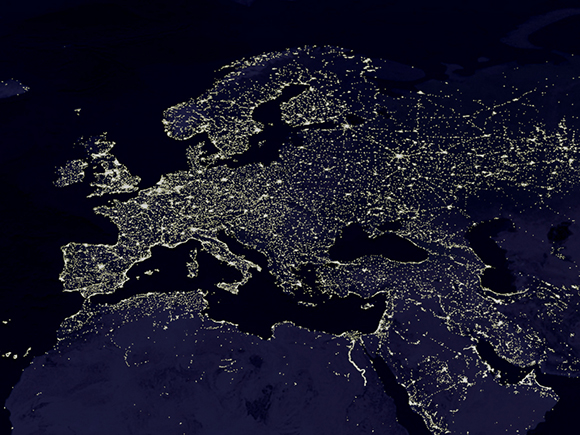
\includegraphics[width=0.7\textwidth]{02_wykresy/europe-nightlights-580.jpg}
\end{center}
\caption{Europa na nocnym zdjęciu satelitarnym}
\small{Żródło: \url{https://visibleearth.nasa.gov/view.php?id=55167}}
\label{fig:ntl}
\end{figure}

Dane NTL mogą zostać wykorzystane do pomiaru ubóstwa \citep{ntl2009}. Autorzy cytowanego artykułu dokonali oszacowania poziomu niedostatku dla wszystkich krajów świata w~ujęciu regionalnym. W Polsce obowiązywał wówczas podział na 49 województw i według mapy zamieszczonej na stronie projektu (\url{https://maps.ngdc.noaa.gov/viewers/dmsp/poverty.html}), wyznaczony wskaźnik ubóstwa nie przekraczał 30\%. Z kolei w Szwecji zweryfikowano istnienie korelacji pomiędzy danymi NTL, a innymi wskaźnikami ekonomicznymi. W przeprowadzonych badaniach wykazano, że istnieje silna zależność pomiędzy gęstością zaludnienia, a nocnym oświetleniem. W przypadku takich wskaźników jak odsetek zatrudnionych czy wielkość płacy korelacja była słabsza \citep{ntl2015}. 

Niestatystyczne źródło danych, pomocne przy analizie i ocenie poziomu ubóstwa, mogą stanowić informacje pozyskane z serwisów zawierających mapy, takich jak: Google Maps czy Open Street Map. Korzystając z API (interfejs programistyczny aplikacji) tych serwisów można pozyskać dane dotyczące obiektów użyteczności publicznej na danym obszarze takich jak np. szpitale, szkoły, supermarkety, itp. Ponadto serwisy te umożliwiają wyznaczenie odległości pomiędzy dwoma punktami uwzględniając rzeczywisty dystans drogowy. Może zostać także podany przybliżony czas podróży w zależności od wybranego środka transportu. Pozyskane dane można pobrać w formacie JSON lub XML i następnie przetwarzać. 

Źródła te nie są jednak wolne od wad. Przede wszystkim nie ma możliwości pobrania informacji historycznych --- można pozyskać wyłącznie aktualny stan bazy. Ponadto API Google Maps umożliwia wysłanie 2,5 tys zapytań dziennie, co w przypadku szczegółowych analiz przestrzennych może nie być wystarczające. Każde kolejne 1000 zapytań to koszt 0,50 dolara. Alternatywą może być wykorzystanie Open Street Map, które takich ograniczeń nie ma, ale z racji tego, że ten serwis jest rozwijany przez użytkowników i każdy może dodawać i usuwać obiekty topograficzne, pozyskane dane mogą być obarczone błędami.

Pobieranie danych ze źródeł internetowych w przypadku, kiedy nie istnieje API jest także możliwe dzięki zastosowaniu automatycznej ekstrakcji danych z sieci --- \textit{web-scrapingu}. Technika ta polega na napisaniu programu, który na podstawie znanej struktury strony internetowej zbiera wymagane informacje w zestandaryzowanej formie. W ten sposób można pozyskiwać dane z~zakresu m.in. cen produktów oraz rynku nieruchomości \citep{beresewicz2015}.

\section{Podsumowanie}

W rozdziale dokonano charakterystyki wykorzystywanych oraz potencjalnych źródeł informacji na temat ubóstwa. W pierwszej kolejności przedstawiono badania reprezentacyjne, w których respondenci między innymi deklarują wysokość dochodów lub wydatków. Ta informacja stanowi podstawę szacowania poziomu ubóstwa w Polsce i jest dostępna w czterech badaniach reprezentacyjnych. Dwa z nich realizowane są rokrocznie (BBGD i EU-SILC), Badanie Spójności Społecznej w cyklu czteroletnim, a Diagnoza Społeczna w dwuletnim. Wielkość próby tych badań umożliwia uzyskanie precyzyjnych oszacowań w bardzo ogólnych przekrojach terytorialnych --- najbardziej szczegółowym poziomem dostępności wyników są województwa.

Druga część rozdziału dotyczy spisów powszechnych. Jest to najpopularniejsze źródło zmiennych pomocniczych w estymacji pośredniej. Zbadanie wszystkich osób żyjących w Polsce w 2002 roku oraz odpowiednia duża próba stanowiąca 20\% populacji w NSP 2011 umożliwiły obserwację charakterystyk ludności, gospodarstw domowych, rodzin i mieszkań na poziomie powiatów. Niestety ze względu na duży koszt organizacji spisów powszechnych odbywają się one co dekadę.

Przeanalizowano także zakres danych zebranych w systemach informacyjnych Ministerstwa Finansów (MF) oraz Ministerstwa Pracy i Polityki Społecznej (MPiPS) w kontekście estymacji ubóstwa. MF w rejestrze PIT dysponuje danymi o dochodach podatników wraz z identyfikatorem terytorialnym. Dane te wykorzystywane są przez GUS w badaniu \textit{Wynagrodzenia w gospodarce narodowej} \citep{pbs2015}. Rejestr ten jednak mógłby być użyty także w badaniach nad ubóstwem ludności. Z kolei MPiPS dysponuje systemami wspomagającymi działania w obrębie bezrobocia rejestrowanego oraz świadczeń pomocy społecznej. W obu przypadkach zakres gromadzonych danych jest bardzo duży. Część z tych informacji w formie zagregowanej jest publikowana przez GUS. Są to m.in. informacje na temat bezrobocia rejestrowanego według różnych przekrojów rzeczowych i terytorialnych oraz wskaźniki korzystania z pomocy społecznej. Dane dostępne są na poziomie gmin. Niemniej liczba cech znajdująca się w tych rejestrach zachęca do przeprowadzenia bardziej szczegółowych analiz z wykorzystaniem np. modeli regresyjnych. Należy przy tym pamiętać, że rejestry administracyjne nie są źródłami statystycznymi co oznacza, że stosowane definicje i warianty cech mogą się różnić od tych stosowanych w systemach statystycznych \citep{roszka2012}.

Poruszono także kwestię pozyskania zmiennych dla statystyki małych obszarów z wykorzystaniem niestatystycznych źródeł. Można tutaj wyróżnić dane pochodzące ze zdjęć satelitarnych, a~także z Internetu (określanych często mianem \textit{Big Data}). Prowadzone badania pokazują wykorzystanie w estymacji pośredniej danych np. z Twittera. Innym źródłem mogą być mapy zawierające informacje o obiektach topograficznych znajdujących się na danym terenie, które można pobrać z wykorzystaniem API. W przypadku braku odpowiedniego interfejsu do pozyskania odpowiednich cech może służyć technika \textit{web-scrapingu}.